\chapter{Governing parameters of  fluid-elastic galloping}
\label{chap:goven_para}

\section{Introduction}

This chapter contains the formulation of non dimensional governing parameters namely, the combined mass-stiffness \massstiff \ and the combined mass-damping \massdamp \ and the results and discussion demonstrating the influence of them. These parameters are formulated by obtaining the relevant time-scales of the system followed by non-dimesnionlising the governing QSS oscillator equation.  

A comparison of Quasi-steady state data presented using the classical VIV parameters and the newly formulated \massstiff \ and \massdamp is presented and it is concluded that \massdamp provides a better collapse for velocity amplitude and mean power compared the classical reduced velocity (\ustar) particularly because unlike \ustar, \massdamp \ does not include a frequency component in it. This is followed by the presentation of QSS data and discussion on the influence of \massstiff \ and \massdamp \ on power, which concludes that the power transfer is a primary function of \massdamp \ and a weak function of \massstiff.

Following this, a comparison of the QSS data with Direct Numerical Simulations (DNS) is presented. This reveals that the power transfer of the DNS data is strongly influenced by both \massstiff \ and \massdamp. Further analysis reveals that there is a good agreement between QSS and DNS for velocity and power at substantially high \massstiff\. As \massstiff \ decreases, the deviation (between QSS simulations and DNS) increases. Power spectral analysis of the DNS data shows a significant response at the vortex shedding at low \massstiff. The relative strength was found out to be an inverse function of \massstiff, which provides a clear explanation for the deviation between QSS simulations and DNS data at low \massstiff. This is primarily due to the influence of vortex shedding where this effect is not accounted in the QSS model.


\section{Formulation of the non-dimensionalised parameters \massstiff \ and \massdamp }
\label{sec: pi_1,pi_2_formulation}

The natural time scales of the system could be obtained by linearising the quasi-steady equation of motion. (Eq:\KJ{equation of motion}) and finding the eigenvalues. The non-linear terms of the forcing function are truncated and the equation of motion could be expressed as, 

\begin{equation}
\label{eqn:eom_linear}
m\ddot{y}{+}c\dot{y}{+}ky{=}\frac{1}{2}\rho U^2 \mathcal{A} a_1\left(\frac{\dot{y}}{U}\right),
\end{equation}

After combining the $\dot{y}$ terms and solving for eigenvalues the following solutions for the eigenvalues could be obtained. 

 \begin{equation}
 \label{eqn:eigs}
 \lambda_{1,2}= -\frac{1}{2}\frac{c-\frac{1}{2}\rho U\mathcal{A}a_1}{m}\pm\frac{1}{2}\sqrt{\left[\frac{c-\frac{1}{2}\rho U\mathcal{A}a_1}{(m)}\right]^2-4\frac{k}{m}}.
 \end{equation} 
 
 Galloping essentially occurs at low frequencies therefore it can be assumed that the spring is relevantly weak and therefore, $k \rightarrow 0$. Hence a single non-zero eigenvalue remains which is, 
  
  \begin{equation}
  \label{eqn:eigs_nospring}
  \lambda=-\frac{c-\frac{1}{2}\rho U\mathcal{A}a_1}{m}.
  \end{equation}
  
  Further, if it is assumed that the mechanical damping is weaker than the fluid dynamic forces on the body the non zero eigenvalue could be further simplified to,
  
 \begin{equation}
 \label{eqn:eigs_nospring_nodamp}
 \lambda=\frac{\frac{1}{2}\rho U\mathcal{A}a_1}{m}.
 \end{equation}  

In this representation $\lambda$ represents the inverse time scale of the motion of the body due to the effect of long-time fluid dynamic forces (or forced due to the induced velocity). This term could also be re-written and $\lambda$ could be expressed as 

\begin{equation}
\label{eqn:timescale}
\lambda = \frac{a_1}{m^*}\frac{U}{D}
\end{equation}

This form clearly shows the significant parameters that influences the inverse time scale of the system. $\partial C_Y / \partial \alpha $, the rate of change in the fluid dynamic force on the body, with respect to the induced angle of attack, is represented by $a_1$. $\frac{U}{D}$ represents the inverse advective time scale of the incoming flow, and the mass ratio is resented by \mstar. Increasing $a_1$ would result in a rapid change of the fluid dynamic force with a small change of the induced angle $\theta$, which is proportional to transverse velocity $\dot{y}$. It can be seen in equation \ref{eqn:timescale} that an increase of $a_{1}$ would result in an increase of the inverse time scale or decrease the response time of the body. In contrast the mass ratio has the opposite effect where an increase in \mstar will lead to a decrease in $\lambda$, since a heavier body (or a body with higher inertia) would have a slower response. 

In order to find the relevant dimensionless groups of the problem, the time scale formulated could be used to non-dimensionalise the equation of motion. The equation of motion presented in Equation \KJ{put final equation of motion} can be non-dimensionalised using the non dimensional time $\tau$, defined as $\tau=t(a_1/m^*)(U/D)$. The non-dimensional equation of motion could then be represented as, 

 \begin{equation}
 \label{eqn:eom_nondim}
 \ddot{Y} + \frac{m^{*2}}{a_1^2}\frac{kD^2}{mU^2}Y = \left(\frac{1}{2} - \frac{m^*}{a_1}\frac{cD}{mU}\right)\dot{Y} - \frac{a_1A_3}{m^{*2}}\dot{Y}^3 + \frac{a_1^3a_5}{m^{*4}}\dot{Y}^5 - \frac{a_1^5a_7}{m^{*6}}\dot{Y}^7.
 \end{equation}
 
 The equation could be further altered by regrouping the coefficients into non-dimenasional groups and could be expressed as, 
 
  \begin{equation}
  \label{eqn:eom_nondim_regroup}
  \ddot{Y} + \frac{4\pi^{2}m^{*2}}{U^{*2}a_1^2}Y = \left(\frac{1}{2} - \frac{c^*m^*}{a_1}\right)\dot{Y} - \frac{a_1A_3}{m^{*2}}\dot{Y}^3 + \frac{a_1^3a_5}{m^{*4}}\dot{Y}^5 - \frac{a_1^5a_7}{m^{*6}}\dot{Y}^7,
  \end{equation}  

\ustar is the reduced velocity which is the typical independent variable ussed in vortex-induced vibration studies. \cstar is the non-dimensional damping parameter which is expressed as $c^*=cD/mU$. 

By analysing equation \ref{eqn:eom_nondim_regroup} it is clear that five dimensionless parameters play a role in setting the response of the system. These are namely the stiffness, damping, mass ratio, the geometry and the Reynolds number. The stiffness is repented by the reduced velocity \ustar, the damping by \cstar and the mass ratio by \mstar. The geometry and the Reynolds number are represented by the coefficients $a_n$, of the polynomial fit to the $C_y$ curve. Using the natural time scales of the system, grouping of these non-dimensional parameters into two groups in the non-dimensional equation of motion, suggests that there are two groups that governs the response which are: $\Gamma_1 = 4\pi^2m^{*2}/U^{*2}a_1^2$ and $\Gamma_2 = c^*m^*/a_1$. $\Gamma_1$ could be described as a combined mass-stiffness, where $\Gamma_2$ could be expressed as a combined mass-damping parameter for a given geometry and a Reynolds number. It is assumed that the stiffness plays a minor role, $\Gamma_2$ seems more likely parameter to collapse the data. The wind tunnel data in the classic paper of galloping by \citep{Parkinson1964} adopted a parameter similar to $\Gamma_2$ to collapse the data. 

All of the quantities that formulate $\Gamma_1$ and $\Gamma_2$ except $a_1$ in theory, could be obtained before an experiment. However in order to obtain the value of $a_1$ static body experiments are required making it relatively difficult to obtain. Here, the \reynoldsnumber and the geometry remains constant and therefore multiplying $\Gamma_1$ with ${a_1}^2$ and $\Gamma_2$ with $a_1$ suitable parameters could be obtained, and formulate a mass-stiffness parameter $\massstiff =  4\pi^2m^{*2}/U^{*2}$, and a mass-damping parameter defined as $\massdamp = c^*m^*$. Therefore equation \ref{eqn:eom_nondim_regroup} can be written in terms of \massstiff \ and \massdamp. 

  \begin{equation}
  \label{eqn:eom_nondim_regroup_pi_1_pi_2}
  \ddot{Y} + \massstiff Y = \massdamp \dot{Y} - \frac{a_1a_3}{m^{*2}}\dot{Y}^3 + \frac{a_1^3a_5}{m^{*4}}\dot{Y}^5 - \frac{a_1^5a_7}{m^{*6}}\dot{Y}^7,
  \end{equation} 
  
From equation \ref{eqn:eom_nondim_regroup_pi_1_pi_2}, it is clear that the governing parameters of the non dimensionlised equation are \massstiff \ \massdamp and \mstar. However, form closer inspection it is possible to see that \mstar has an impact on the non-linear terms of the forcing function. The velocity pf the and hence the induced angle of attack needs to be very high in order for the non-linear terms to be applicable. 

\section{Quasi-steady state results}
\label{sec:qss_results} 

\subsection{Classical VIV parameters vs. \massstiff \ and \massdamp.}
\label{subsec:compare_data}


Vortex-induced vibrations being another form fluid-structure interaction which occurs in a slender structure, has been investigated as candidate for power extraction from external flows. Significant progress on this problem have been made by \cite{Bernitsas2008a-concept,Bernitsas2009,Raghavan2010a,Lee2011b} and other colleagues in VIVCACE group in the University of Michigan. Hence, it may seem that it is reasonable to present the data in a fluid-elastic problem using the same parameters in a VIV problem.

\begin{figure}
  \setlength{\unitlength}{\textwidth}
  \fbox{
  \begin{picture}(1,0.9)(0,0)
    % % %90
      % % % Parkinson Data 
      \put(0.035,0.5){\includegraphics[width=0.5\unitlength]{../FnP/gnuplot/displacement_amp_re200.eps}}
      \put(0.035,0.27){\includegraphics[width=0.5\unitlength]{../FnP/gnuplot/velocity_amp_re200.eps}}
      \put(0.035,0.02){\includegraphics[width=0.5\unitlength]{../FnP/gnuplot/mean_power_re_200.eps}}
      
      \put(0.495,0.27){\includegraphics[width=0.5\unitlength]{../FnP/gnuplot/velocity_amp_collapsed_re200.eps}} 
      \put(0.495,0.02){\includegraphics[width=0.5\unitlength]{../FnP/gnuplot/mean_power_collapsed_re_200.eps}}
      \put(0.495,0.5){\includegraphics[width=0.5\unitlength]{../FnP/gnuplot/displacement_amp_collpased_re200.eps}}
      
%      \put(0.23,0.00){ $\displaystyle\frac{c}{\rho\mathcal{A}U}$}
%      \put(0.73,0.00){ $\displaystyle\frac{c}{\rho\mathcal{A}U}$}

      \put(0.28,0.00){\ustar}
      \put(0.78,0.00){\massdamp}
      
      \put(0.01,0.405){$\displaystyle\frac{V}{D}$}\
       \put(0.01,0.63){$\displaystyle\frac{A}{D}$}
      
      \put(-0.02,0.13){$\displaystyle\small\frac{P_{m}}{\rho \mathcal{A}U^3 }$}
      
      \put(0.093,0.705){\small(a)}
      \put(0.555,0.705){\small(b)}
      \put(0.093,0.475){\small(c)}
      \put(0.555,0.475){\small(d)}
      \put(0.093,0.225){\small(e)}
      \put(0.555,0.225){\small(f)}

  \end{picture}
}
  \caption{Displacement amplitude, velocity amplitude and mean power data as functions of two different independent varibles. Data presented in (a), (c) and (e) using the classical VIV parameter $\ustar$, obtained at $Re=200$ and $m^*=20$ at three different damping ratios: $\zeta=0.075$ ($\times$), $\zeta=0.1$ (\ding{117}) and $\zeta=0.15$ (+). (b) (d) and (f)  are the same data presented using the combined mass-damping parameter (\massdamp) as the independent variable.  }
  \label{fig:compare_data}
\end{figure}

QSS data presented in figure \ref{fig:compare_data} at $\reynoldsnumber=200$, shows a comparison between classical VIV and the newly formulated parameters presented as independent variables. The displacement amplitude, velocity amplitude and the mean power is presented in sub-figures (a), (c) and (e), as functions of the classical VIV parameter \ustar for different $\zeta$. The same data as functions of \massdamp, are presented in sub-figures (b), (d) and (f), for various, reasonably high values of \massstiff \KJ{put the parameters used section}. Sub-figure (e) shows a similar trend to \cite{Barrero-Gil2010a}. The Value of the peak power remains constant. However, the power curve shifts to the right as $\zeta$ is increased. Here, in figure \ref{fig:compare_data} the maximum dimensionless power is achieved at two times the velocity at which the galloping starts, which is similar to the observations made by \citet{Barrero-Gil2010a,vicente-Ludlam2014}. An excellent collapse for velocity amplitude and mean power could be observed on the data, presented using the dimensionless group \massdamp, formulated using the natural time scales of the system. This implies that essentially velocity amplitude and the mean power is dictated by \massdamp which furthermore, implies that the natural frequency of the system which is used to scale \ustar, $\zeta$ and \massstiff does not have a significant influence on the behaviour of the system, unlike VIV, which is a resonant phenomenon.  
 

\subsection{High and low \reynoldsnumber \ data}
\label{subsec:high_Re_data}

% !TeX spellcheck = en_GB
\begin{figure}
  \setlength{\unitlength}{\textwidth}

        \begin{picture}(1,0.3)(-0.02,0)

      % % % Parkinson Data 
%      \put(0.025,0.5){\includegraphics[width=0.5\unitlength]{../FnP/gnuplot/displacement_amp_collapsed_parkinson.eps}}
%      \put(0.025,0.27){\includegraphics[width=0.5\unitlength]{../FnP/gnuplot/velocity_amp_collapsed_parkinson.eps}}
%      \put(0.495,0.27){\includegraphics[width=0.5\unitlength]{../FnP/gnuplot/velocity_amp_collapsed_re200.eps}}
      
      \put(0.025,0.02){\includegraphics[width=0.5\unitlength]{../FnP/gnuplot/mean_power_collapsed_parkinson.eps}}
      \put(0.495,0.02){\includegraphics[width=0.5\unitlength]{../FnP/gnuplot/mean_power_optimum_re_200.eps}}
%      \put(0.495,0.5){\includegraphics[width=0.5\unitlength]{../FnP/gnuplot/displacement_amp_collpased_re200.eps}}
      
%      \put(0.23,0.00){ $\displaystyle\frac{c}{\rho\mathcal{A}U}$}
%      \put(0.73,0.00){ $\displaystyle\frac{c}{\rho\mathcal{A}U}$}

      \put(0.28,0.00){\massdamp}
      \put(0.74,0.00){\massdamp}
      
     
       \put(-0.03,0.13){$\displaystyle\frac{P_{m}}{\rho \mathcal{A}U^3 }$}
      

      \put(0.095,0.218){\small(a)}
      \put(0.565,0.218){\small(b)}
      
    \end{picture}

  \caption{Mean power as a function of \massdamp. Data presented at (a) $\reynoldsnumber=22300$, $\massstiff=200$ ($\times$), $massstiff=2000$ (\ding{117}) and $\massstiff=10000$ (+). (b) $\reynoldsnumber=200$, $\massstiff=100$. Hysteresis could be observed at high \reynoldsnumber  }
    \label{fig:collapsed_data}
\end{figure}

 %vspace{10cm}


The successful collapse of data, mean power in particular using \massdamp for low Reynolds number ($\reynoldsnumber=200$), could be replicated at high Reynolds numbers. An example case is presented in figure \ref{fig:compare_data} at $\reynoldsnumber=22300$ for selected vales of \massstiff. The successful collapse of mean power data at high Reynolds numbers shows that suitability of using \massdamp \ as an independent variable across a large range of Reynolds numbers. 

Hysteresis is evident in the high Reynolds number case ($\reynoldsnumber=22300$). Manipulating the initial condition (initial displacement) lead to obtaining different solutions for the same \massdamp \ value. The upper and lower branch were obtained by giving an initial displacement which was higher than the expected amplitude and providing a lower initial displacement respectively. Even though in theory, there is a possibility of a third state, this unstable branch could not be achieved with a time integration method (also observed by \citep{Vio2007}) such as the one employed in this study.

\subsection{Dependence on mass-stiffness, \massstiff}
\label{subsec:dependence pi_1}

\begin{figure}
  \setlength{\unitlength}{\textwidth}
\fbox{
        \begin{picture}(1,1.1)(0,0.35)

      % % % Parkinson Data 
      \put(0.09,1.1){\includegraphics[width=0.757\unitlength]{../FnP/gnuplot/displacement_high_pi_1.eps}}
      \put(0.1,0.75){\includegraphics[width=0.75\unitlength]{../FnP/gnuplot/velocity_high_pi_1.eps}}
      \put(0.1,0.35){\includegraphics[width=0.75\unitlength]{../FnP/gnuplot/mean_power_high_pi_1.eps}}
      
         \put(0.07,0.95){$\displaystyle\frac{V}{D}$}\
         \put(0.07,1.3){$\displaystyle\frac{A}{D}$}
         \put(0.05,0.6){$\displaystyle\frac{P_{m}}{\rho \mathcal{A}U^3 }$}



%      
%      \put(0.45,0.7){\small(a)}
%      \put(0.926,0.7){\small(b)}
%      \put(0.726,0.45){\small(c)}
%  

      
    \end{picture}
}
  \caption{QSS data at high \massstiff \ levels. (a) displacement amplitude, (b) velocity amplitude and (c) mean power as a function of \massdamp. Data presented at four different combined mass-stiffness levels.\ $\massstiff=10 \ (\mstar=20,\ \ustar \approx 40)$ \ (\ding{117}),\ $\massstiff=100 \ (\mstar=130,\ \ustar \approx 80) \ (+)$ and \ $\massstiff=1000 \ (\mstar=400,\ \ustar \approx 40) \ (\triangle)$}
    \label{fig:high_pi_1}
\end{figure}

 %vspace{10cm}


From the results of sections \ref{subsec:compare_data} and \ref{subsec:high_Re_data} shows essentially a single variable governs the mean extracted power, which is the combined mass-damping parameter, \massdamp. The time scale analysis carried out in  section \ref{sec: pi_1,pi_2_formulation} shows that not only \massdamp \ but also \massstiff influences the system. Previous studies such as \cite{bouclin:77} have also reported a complex interaction between the displacement amplitude and the natural frequency, for high natural frequencies in particular; or in this instance equivalent to low values of \massstiff.  This section investigates the impact of \massstiff further. The overall behavior of the system is divided into two regimes, one for ``high" \massstiff \ and the other for ``low" \massstiff and analysed.

The mean power as a function of \massdamp \ for a range of values of \massstiff is presented in figure \ref{fig:high_pi_1}. In the two subfigures presented, (a) shows the data for $\massstiff \geq 10$, while (b) shows data for $\massstiff \leq 10$.  The excellent collapse in figure \ref{fig:high_pi_1}(a) shows that for $\massstiff \geq 10$, the mean power is independent of \massstiff.

In contrast figure \ref{fig:high_pi_1}(b) shows that for low values of $\massstiff \leq 10$, the predicted mean power increases as \massdamp \ decreases. This indicates that at this region ($\massstiff < 10$), the mean power is a weak function of \massstiff; hence, providing a distinction between high and low regimes of \massstiff. The mean extracted power is only a function of \massdamp \ where $\massstiff \geq 10$ or for high \massstiff. For low values, $\massstiff < 10$, the mean power becomes a strong function of \massdamp \ and a weak function of \massstiff.

It is clear that regardless of the value of \massstiff, the variation of power with \massdamp \ is essentially the same. As \massdamp \ is increased, the mean extracted power will increase to the point which, it will attain some maximum value and then decrease. This relationship between power and \massdamp \ could be explained by analysing the time histories of selected cases. 
AS an example, data at $\massstiff=10$, $m^*=20$ and $\reynoldsnumber=200$ are presented in figure \ref{fig:power_time_histories}. Three major regions where the value of the power curve are considered. These regions are \massdamp\ less than (region 1), equal to (region 2) and greater than (region 3) to the \massdamp\ value where the mean power is at its maximum.

\begin{figure}

  \setlength{\unitlength}{\textwidth}
%  \fbox{
  \begin{picture}(1,0.58)(0,0.35)
    % % % 90
    \put(0.03,0.76){\includegraphics[width=0.35\unitlength]{../FnP/gnuplot/power_time_history_015.eps}}
    \put(0.03,.58){\includegraphics[width=0.35\unitlength]{../FnP/gnuplot/f_y_history_015.eps}}
    \put(0.03,0.4){\includegraphics[width=0.35\unitlength]{../FnP/gnuplot/theta_time_history_015.eps}}
    
    % % 165
    \put(0.36,0.76){\includegraphics[width=0.35\unitlength]{../FnP/gnuplot/power_time_history_54.eps}}
    \put(0.36,.58){\includegraphics[width=0.35\unitlength]{../FnP/gnuplot/f_y_history_54.eps}}
    \put(0.36,0.4){\includegraphics[width=0.35\unitlength]{../FnP/gnuplot/theta_time_history_54.eps}}
    
    \put(0.68,0.76){\includegraphics[width=0.35\unitlength]{../FnP/gnuplot/power_time_history_08.eps}}
    \put(0.68,.58){\includegraphics[width=0.35\unitlength]{../FnP/gnuplot/f_y_history_08.eps}}
    \put(0.68,0.4){\includegraphics[width=0.35\unitlength]{../FnP/gnuplot/theta_time_history_08.eps}}
    
    \put(0.55,0.36){$\displaystyle{\frac{tU}{D}}$}
    \put(0.2,0.36){$\displaystyle{\frac{tU}{D}}$}
    \put(0.85,0.36){$\displaystyle{\frac{tU}{D}}$}
    
    \put(0.0,0.87){$\frac{P}{\rho \mathcal{A}U^3}$}
    \put(0.01,0.66){$F_y$}
    \put(0.01,0.49){$\theta$}
    
    \put(0.08,0.76){(a)}
    \put(0.08,0.58){(d)}
    \put(0.08,0.38){(g)}
    
    \put(0.4,0.76){(b)}
    \put(0.4,0.58){(e)}
    \put(0.4,0.38){(h)}
    
    \put(0.72,0.76){(c)}
    \put(0.72,0.58){(f)}
    \put(0.72,0.38){(i)}
  \end{picture}
%}
  \caption{Time histories of $P_t$, $P_d$, $F_y$ and $\theta$ at $\massdamp=0.15$, $0.54$ and $0.8$ from the QSS model. Data was obtained at $m^*=20$, $\massstiff=10$ and \reynoldsnumber=200. The time histories of $P_t$ ( \solidrule[4mm]\hspace{1mm}) and $P_d$ (\protect\dashedrule) are presented for: (a) $\massdamp= 0.15$; (b) $\massdamp= 0.54$; (c) $\massdamp= 0.8$. Time histories of the instantaneous force $F_y$ for: (d) $\massdamp= 0.15$; (e) $\massdamp= 0.54$; (f) $\massdamp= 0.8$. Time histories of the instantaneous angle $\theta$ for: (g) $\massdamp= 0.15$; (h) $\massdamp= 0.55$; (i) $\massdamp= 0.8$.}
  \label{fig:power_time_histories}
\end{figure}






The damping is low is low in region 1 ($\massdamp=0.15$) in comparison with region 2 and 3. Although this may lead to larger oscillations, according to equation \ref{eqn:power} damping is required to dissipate and therefore extract power. Hence, a low mean power output is gained at low damping. The high velocity amplitude leads the equivalent incident angle $\theta$ to exceed the positive range of $C_y$ (i.e. $0<\theta<6^\circ$ as shown in figure\ref{cy ploynomial}(a)) resulting a negative dissipated power by damping $P_d$ over some portion of the cycle as shown in figure \ref{fig:power_time_histories} (a). The galloping force $F_y$ and the transverse velocity $\dot{y}$ are not in phase in this portion of the cycle where the force opposes the direction of travel. As a consequence, during this period of time the opposite of what is expected happens, where the power is transferred from the structure to the fluid. Since \massdamp \ is substantially low, from an energy perspective, the mechanical damping is not sufficient to remove the energy transferred from the fluid to the structure through work during other times of the cycle. Hence, as depicted by the negative region of $P_d$, this excess energy is transferred back to the fluid.



A clear sinusoidal signal of both $P_d$ and $P_t$ (\ref{fig:power_time_histories}(c)) could be observed at region 3 where $\massdamp=0.8$ and the damping constant is high. The equivalent incident angle $\theta$ (which for small values, is proportional to the transverse velocity of the body) is in phase with the galloping force $F_y$ as shown in figures \ref{fig:power_time_histories}(f) and  \ref{fig:power_time_histories}(i). The velocity amplitude is small in this case resulting $\theta$ falling within the rage where the fluid-dynamic force ($F_y$) increases within the incident angle (i.e. $0<\theta \leq 5^\circ$ as shown in figure \ref{fig:lift_curves}(a)). These conditions are favourable for high power output according to equation \ref{power_alt}. Be that as it may, in this case the velocity is limited because of the high damping resulting relativity low fluid dynamic forcing. 

A harmony between the high and low values of damping could be found at region 2  ( $\massdamp=0.54$). It is evident that $P_d$ remains periodic but is not a pure sinusoidal signal. Two `peaks' are present in a single half cycle from the time history graph of $P_d$ as shown in figure \ref{fig:power_time_histories}(b). The velocity amplitude actually exceeds the equivalent incident angle where the fluid-dynamic forces peaks (i.e. $\theta=5^\circ$ in \ref{cy ploynomial} (a)) in this scenario. The dip in between the two peaks in a single half cycle correspond approximately to the time where the transverse velocity is higher that 0.09 and $F_y$ is decreasing with increasing transverse velocity. As this region is the best compromise between region 1 and region 3, the maximum mean power could be attained in this region. Region 2 could also be identified as the ``sweet spot" for energy extraction as the damping is high enough to obtained a high power output while not so high for the motion to be completely suppressed. 


\subsection{Dependence on the mass ratio \mstar}
\label{sec:chp-pi_1_pi2_mstar}


It is clear that the mean extracted power is only a function of \massdamp \ for high values of \massstiff. However, the question remains about the region of low \massstiff. Does the variation of the mean extracted power occur purely as a function of \massstiff, or does the mass ratio also has an influence on power? The QSS model was solved by varying the values for \mstar
but keeping the \massstiff fixed. In other words \massstiff\ was changed by changing the stiffness of the system. 
 
It is clear from figure \ref{fig:low_pi_1}, data presented being the mean extracted power  as a function of \massdamp, for a fixed $\massstiff = 0.1$, for three different values of \mstar, that mean power is independent of \mstar, hence, it is only a function of \massstiff\ and \massdamp.

\begin{figure}
  \setlength{\unitlength}{\textwidth}

        \begin{picture}(1,0.4)(0,0.4)

      % % % Parkinson Data 
%      \put(0.1,1.1){\includegraphics[width=0.75\unitlength]{../FnP/gnuplot/displacement_low_pi_1.eps}}
%      \put(0.1,0.76){\includegraphics[width=0.75\unitlength]{../FnP/gnuplot/velocity_low_pi_1.eps}}
      \put(0.1,0.42){\includegraphics[width=0.75\unitlength]{./chapter-pi_1_pi_2/FnP/gnuplot/mean_power_low_pi_1.eps}}
      
%       \put(0.07,0.95){$\displaystyle\frac{V}{D}$}
%       \put(0.07,1.3){$\displaystyle\frac{A}{D}$}
       \put(0.05,0.6){$\displaystyle\frac{P_{m}}{\rho \mathcal{A}U^3 }$}
       \put(0.5,0.4){$\massdamp$}
       \
%\put(0.189,1.415){\small(a)}
%\put(0.189,1.07){\small(b)}
%\put(0.189,0.73){\small(c)}

%  

      
    \end{picture}

  \caption{Dimensionless mean power as a function of \massdamp\ obtained using QSS model at \ $\massstiff=0.1$.  Data presented at  $\mstar=2$ (\ding{117}), \  $ \mstar=20 \ (\triangle)$ and  $ \mstar=50 \ (*)$. The mass ratio does not have an effect on \massstiff \ even at low \massstiff.}
    \label{fig:low_pi_1}
\end{figure}

 %vspace{10cm}



\subsection{Comparison with DNS data}
\label{sec:chp-pi_1_pi2_dns}

The main drawback of the QSS model is that the instantaneous lift generated by the induced velocity is the only driving force of the system. However, in realistic scenarios the flow is far more complex and the only force affecting the system is not the induce lift. Force generated due to vortex shedding is one of the prominent forces in these systems. Hence, when the QSS model is being used, one of the essential assumptions is that the effect of vortex shedding is minimal. Due to this reason the model has been always used at high Reynolds numbers and at high \mstar. Therefore, a study to identify the limiting parameters of the QSS model at low Reynolds numbers was carried out  using a comparison of QSS data with DNS results.


% % % % % % % % % % % % % % % % % % % % % % % % % % 

A sinusoidal forcing function was introduced to the QSS model in order to account for the forcing by vortex shedding by \citet{Joly2012}. In this study displacement data obtained by the QSS model and the DNS simulations were compared which agreed well at low Reynolds numbers. The data were obtained at zero damping levels. As the primary focus of this study is the behaviour and the power transfer of the system, analysing the behaviour of the system with increasing damping is of interest.   

Figure \ref{fig:qss_fsi} provides a comparison between QSS and the DNS results.The maximum displacement, velocity and mean extracted power are presented as a function of \massdamp. A range of values of \massstiff\ are compared to the QSS model data for $\massstiff = 10$. Only little variation with \massstiff \ could be found in  the displacement amplitude (figure\ref{fig:qss_fsi}(a)) and velocity amplitude (\ref{fig:qss_fsi}(b)). Thus the comparison between the QSS model and the DNS simulation is quite satisfactory for these two quantities. In contrast, there is a significant influence of both \massstiff\ and \massdamp\ on the mean extracted power which is  presented in figure \ref{fig:qss_fsi}(c). This discrepancy become more vivid in the regions where the value of \massstiff\ is low. These regions has the largest discrepancy between the QSS model and DNS data. A comparison of data between figures \ref{fig:qss_fsi}(c) and \ref{fig:high_pi_1}(a) shows that \massstiff has a much more significant influence on the extracted power than the predictions by the QSS model for low \massstiff\ values. Indeed as discussed in section \ref{subsec:dependence pi_1} the QSS model predicts that the mean extracted power should increase with decreasing \massstiff\ when \massstiff\ moves to the low \massstiff\ region (figure \ref{fig:high_pi_1}(b)). However, the DNS data show sort of an opposite result where the extracted mean power decreases with decreasing \massstiff.


\begin{figure}
  \setlength{\unitlength}{\textwidth}

        \begin{picture}(1,1.1)(0,0.35)

      % % % Parkinson Data 
      \put(0.1,1.1){\includegraphics[width=0.75\unitlength]{./chapter-pi_1_pi_2/FnP/gnuplot/fqss_fsi_displace.eps}}
      \put(0.1,0.737){\includegraphics[width=0.75\unitlength]{./chapter-pi_1_pi_2/FnP/gnuplot/qss_fsi_velocity.eps}}
      \put(0.1,0.38){\includegraphics[width=0.75\unitlength]{./chapter-pi_1_pi_2/FnP/gnuplot/qss_fsi_power.eps}}
      
      



%      
    \put(0.15,1.41){\small(a)}
     \put(0.15,1.05){\small(b)}
     \put(0.15,0.69){\small(c)}
\put(0.03,0.95){$\displaystyle\frac{V}{U}$}
\put(0.03,1.3){$\displaystyle\frac{A}{D}$}
\put(0.0,0.56){$\displaystyle\frac{P_{m}}{\rho \mathcal{A}U^3 }$}
\put(0.466,0.35){$\massdamp$}

      
    \end{picture}

    \caption{Comparison of data generated using the quasi-static model
      and full DNS simulations at (a) Displacement amplitude, (b)
      velocity amplitude and (c) dimensionless mean power as functions of
      \massdamp. Data were obtained at $\reynoldsnumber = 200$ at four
      values $\massstiff=10$ ($\mstar= 20.13$) (\ding{83}),
      $\massstiff=60$ ($\mstar =49.31$) (\ding{108}), $\massstiff=250$
      ($\mstar= 100.7$) ($\triangle$) and $\massstiff=1000$ ($\mstar=201.3$) (\ding{117}). The QSS data at $\massstiff=10$ \
      (\protect\dashedrule).}
    \label{fig:qss_fsi}
\end{figure}

 %vspace{10cm}



% % % % % % % % % % % % % % % % % % % %

The dependence of the mean extracted power on \massstiff\ is clearly shown in figure \ref{fig:max_power}(a).  Here, the maximum power extracted for a given value of \massstiff, over all values of \massdamp (essentially the value of extracted power at the turning point), is plotted as a function of \massstiff. A quadratic fit was used obtain these values presented in figure \ref{fig:low_pi_1} and finding the mean extracted power at the turning point of the power curve. It is clear that there is a rapid decrease in extracted power as $\massstiff \rightarrow 0$. 

% !TeX spellcheck = en_GB
\begin{figure}
  \setlength{\unitlength}{\textwidth}
  \begin{picture}(1,0.3)(-0.02,0)
          
    \put(0.025,0.04){\includegraphics[width=0.45\unitlength]{../FnP/gnuplot/p_max.eps}}
    \put(0.54,0.04){\includegraphics[width=0.45\unitlength]{../FnP/gnuplot/p_2_p_max.eps}}
        
    \put(0.48,0.07){ \rotatebox{90}{$\displaystyle\massdamp$ \scriptsize{at max power}} }
    \put(-0.07,0.16){$\displaystyle\frac{P_{max}}{\rho \mathcal{A}U^3 }$}
    % \put(0.73,0.00){ $\displaystyle\frac{c}{\rho\mathcal{A}U}$}

    \put(0.24,0.00){\massstiff}
    \put(0.75,0.00){\massstiff}
   
    \put(0.058,0.07){\small(a)}
    \put(0.57,0.07){\small(b)}
      
    \end{picture}

    % \caption{Comparison of DNS data. (a) Maximum power obtained using
    %   a 3 point localised quadratic fitting as a function of
    %   \massstiff. (b) \massdamp as a function of \massstiff at maximum
    %   power}

    \caption{(a) Maximum power of QSS data ($\circ$) and DNS data ($\bullet$), and (b) the value of \massdamp\ 
        where maximum power occurs in DNS data, as functions of \massstiff.
           The maximum power asymptotes to an upper
        value with increasing \massstiff, while the value of \massdamp\
        where maximum power occurs is relatively insensitive to
        \massstiff. The maximum power of the DNS data remains relatively constant as shown before. The dash curve (\protect\dashedrule) of (a) follows the logarithmic fit of the maximum power which is $f(x)=1.48 \times 10^{-4} \ ln(x) + 1.9 \times 10^{-3} $ equation.}

    \label{fig:max_power}
\end{figure}

 %vspace{10cm}


Figure \ref{fig:max_power}(a) also shows that \massstiff\ is important to higher values than predicted by the QSS model. The maximum extracted power is essentially independent of \massstiff\ for for $\massstiff>10$, which could be observed by the open symbols in the figure. Nonetheless a significant dependence on \massstiff\  $\massstiff<250$ could be observed in the extracted power. Yet, as the \massstiff\ increases the mean power converges to that of the values predicted by the QSS model.

The value of \massdamp\ at the turning point  of the power curve or the point of maximum power is shown in figure \ref{fig:max_power}(b). The open symbols represents the values predicted by the QSS model while the values predicted by DNS simulations are represented by the close symbols. These two values does not coincide where the DNS predictions (shown with a dashed line) has a value around $0.41$ while the predictions of the QSS model has a value of $0.5$. Regardless, both QSS model and DNS show that while the mean power is a reasonably strong function of \massstiff, the value of \massdamp\ at the point of maximum power output is relatively unaffected.


The percentage discrepancy between the QSS DNS  extracted power data as a function of \massstiff\ was calculated using equation \ref{eqn:error_calculation} in order to further quantify the performance of the QSS model.  
 
\begin{equation}   \label{eqn:error_calculation} 
\% \ error=\left|{\frac{P_{m(QSS)} - P_{m(DNS)}}{P_{m(DNS)}}}\right| \times 100.
\end{equation}

Figure \ref{fig:error} shows the data obtained by this error calculation along with a power-law best fit $138.697\massstiff^{-0.6}$. It clearly shows that the as \massstiff increases the percentage error between QSS model and DNS is quickly decreases. But, the discrepancy between the two can be quite large, about $30\%$ at low values of \massstiff.

\begin{figure}
  \setlength{\unitlength}{\textwidth}

        \begin{picture}(1,0.4)(0,0.4)

      \put(0.1,0.45){\includegraphics[width=0.75\unitlength]{../FnP/gnuplot/error.eps}}
      
%       \put(0.07,0.95){$\displaystyle\frac{V}{D}$}
%       \put(0.07,1.3){$\displaystyle\frac{A}{D}$}
       \put(0.05,0.58){\rotatebox{90}{$\% \ error$}}
%       \put(0.5,0.4){$\massdamp$}
       \put(0.5,0.4){$\massstiff$}
    \end{picture}

  % \caption{Comparison of maximum power between QSS and DNS data obtained using 3 point local quadratic curve fitting.The error was obtained using Eq:\ref{eqn:error_calculation}}
    \caption{The difference between the maximum power predicted by
        the QSS model for $\massstiff = 10$, and the DNS data as a
        function of \massstiff. The QSS model prediction is worst for
        low values of \massstiff.}
    \label{fig:error}
\end{figure}

 %vspace{10cm}


The influence of vortex shedding could be one of the likely reason for this discrepancy at low \massstiff\ which is not accounted in the QSS model. The frequency spectra of the velocity of the boy from DNS cases at varying \massstiff\  at a value of $\massdamp=0.47$ which is close to the value at which the mean extracted power is a maximum, were plotted to test this hypothesis. Figure \ref{fig:spectrum} shows this power spectrum plots along with the original time histories of the transverse velocities of the body. 

\begin{figure}
  \setlength{\unitlength}{\textwidth}

  \begin{picture}(1,1.2)(0,-0.1)
    % % %90
      % % % Parkinson Data 
      \put(0.005,0.8){\includegraphics[width=0.5\unitlength]{../FnP/gnuplot/spec_20_sig.eps}}
      \put(0.005,0.5){\includegraphics[width=0.5\unitlength]{../FnP/gnuplot/spec_50_sig.eps}}
      \put(0.005,0.27){\includegraphics[width=0.5\unitlength]{../FnP/gnuplot/spec_100_sig.eps}}
      \put(0.005,0.02){\includegraphics[width=0.5\unitlength]{../FnP/gnuplot/spec_200_sig.eps}}
      
      
      \put(0.505,0.8){\includegraphics[width=0.5\unitlength]{../FnP/gnuplot/spec_20.eps}}
      \put(0.505,0.5){\includegraphics[width=0.5\unitlength]{../FnP/gnuplot/spec_50.eps}}
      \put(0.505,0.27){\includegraphics[width=0.5\unitlength]{../FnP/gnuplot/spec_100.eps}} 
      \put(0.505,0.02){\includegraphics[width=0.5\unitlength]{../FnP/gnuplot/spec_200.eps}}
      
      
%      \put(0.23,0.00){ $\displaystyle\frac{c}{\rho\mathcal{A}U}$}
%      \put(0.73,0.00){ $\displaystyle\frac{c}{\rho\mathcal{A}U}$}

      \put(0.28,-0.03){$\displaystyle\frac{fd}{U}$}
      \put(0.78,-0.03){$\displaystyle\frac{tU}{D}$}
      
      \put(0.51,0.405){$\displaystyle\frac{V}{D}$}
      \put(0.51,0.63){$\displaystyle\frac{V}{D}$}
      \put(0.51,0.13){$\displaystyle\frac{V}{D}$}
      \put(0.51,0.93){$\displaystyle\frac{V}{D}$}
      
      \put(0.10,0.995){\small(a)}
      \put(0.625,0.995){\small(b)}
      \put(0.1,0.695){\small(c)}
      \put(0.625,0.695){\small(d)}
      \put(0.1,0.465){\small(e)}
      \put(0.625,0.465){\small(f)}
      \put(0.1,0.217){\small(g)}
      \put(0.625,0.217){\small(h)}

  \end{picture}

  \caption{Velocity signal (right) and the corresponding power spectrum (left) of the DNS data at 3 different \massstiff \ at $\massdamp=0.8$. (a) and (b) $\massstiff=10$, (c) and (d) $\massstiff=60$, (e) and (f) $\massstiff=250$, (g) and (h) $\massstiff=1000$. \ustar \ is kept at 40 therefore the mass ratio increases as \ \massstiff \ increases. It is evident that the influence of vortex shedding reduces as the inertia of the system increases.}
  \label{fig:spectrum}
\end{figure}


% % % % % % % % % % % % % % % % % % % % % %

This figure shows the  velocity signals at $\massstiff=0.8$ and $\massdamp= 10, 60, 250$ and $1000$ and the corresponding spectrum. A significant component around $fd/U=0.156$ which can be identified as the vortex shedding frequency could be seen in the spectral data. As the \massstiff\ increases a clear reduction of the magnitude of the component at the  vortex shedding frequency could be observed. This indecates that the influence of vortex shedding is much more prominent at low \massstiff,  therefore resulting in larger deviations from quasi-steady state results. This builds on the work of \cite{Joly2012}, which was conducted at zero damping, that implied that mean extracted power would be influenced by vortex shedding at low mass.

This influence is explicitly shown here. Figure \ref{fig:spec_pow} plots the relative intensity of the component at the vortex shedding frequency to the component at the galloping or oscillation frequency in the spectra of figure \ref{fig:spectrum}.

\begin{figure}
  \setlength{\unitlength}{\textwidth}

        \begin{picture}(1,0.4)(0,0.4)

      \put(0.1,0.45){\includegraphics[width=0.75\unitlength]{../FnP/gnuplot/spec_pow.eps}}
      
%       \put(0.07,0.95){$\displaystyle\frac{V}{D}$}
%       \put(0.07,1.3){$\displaystyle\frac{A}{D}$}
       \put(0.045,0.43){\rotatebox{90}{$relative \ power \ of \ shedding$ }}
%       \put(0.5,0.4){$\massdamp$}
       \put(0.43,0.4){$\massstiff$}
    \end{picture}

  % \caption{Comparison of maximum power between QSS and DNS data obtained using 3 point local quadratic curve fitting.The error was obtained using Eq:\ref{eqn:error_calculation}}
    \caption{The relative power of the vortex shedding as a fucntion of \massstiff. The relative power of the vortex shedding decreases as \massstiff \ increases. This trend follows $0.977x^{-0.5}$ equation}
    \label{fig:spec_pow}
\end{figure}

 %vspace{10cm}


The relative strength of the vortex shedding is seen to be large at low values of \massstiff and drastically decreases as \massstiff\ is increases. This follows a similar behaviour to the discrepancy between the QSS and DNS mean extracted power shown in figure \ref{fig:error}. From the figure to could be seen that the variation of the relative power of the vortex shedding frequency to the galloping frequency is similar to  $0.977\massstiff^{-0.52}$ 

The difference between the power predicted by the QSS and DNS models scales with $\massstiff^{-0.6}$ while the relative power at the vortex shedding frequency scales with $\massstiff^{-0.52}$. Both these scalings are quite similar which is closer to $1/\sqrt{\massstiff}$. Though it is unequivocal, this correlation is a strong indication that the discrepancy between QSS and DNS is result of the influence of vortex shedding, even though the frequencies of vortex shedding and galloping remains well separated by around similar amount for all values of \massstiff (Figure\ref{fig:spec_pow}). The data presented in figure \ref{fig:spec_pow} also give some sort of an indication of the strength of any vortex shedding correction term that might be added to the QSS model in an effort to decrease the discrepancy between it and the DNS simulations.

\begin{figure} [!htb]
  \setlength{\unitlength}{\textwidth}
  \begin{picture}(1,1.1)(0,0.66)
    
    \put(0,1.5){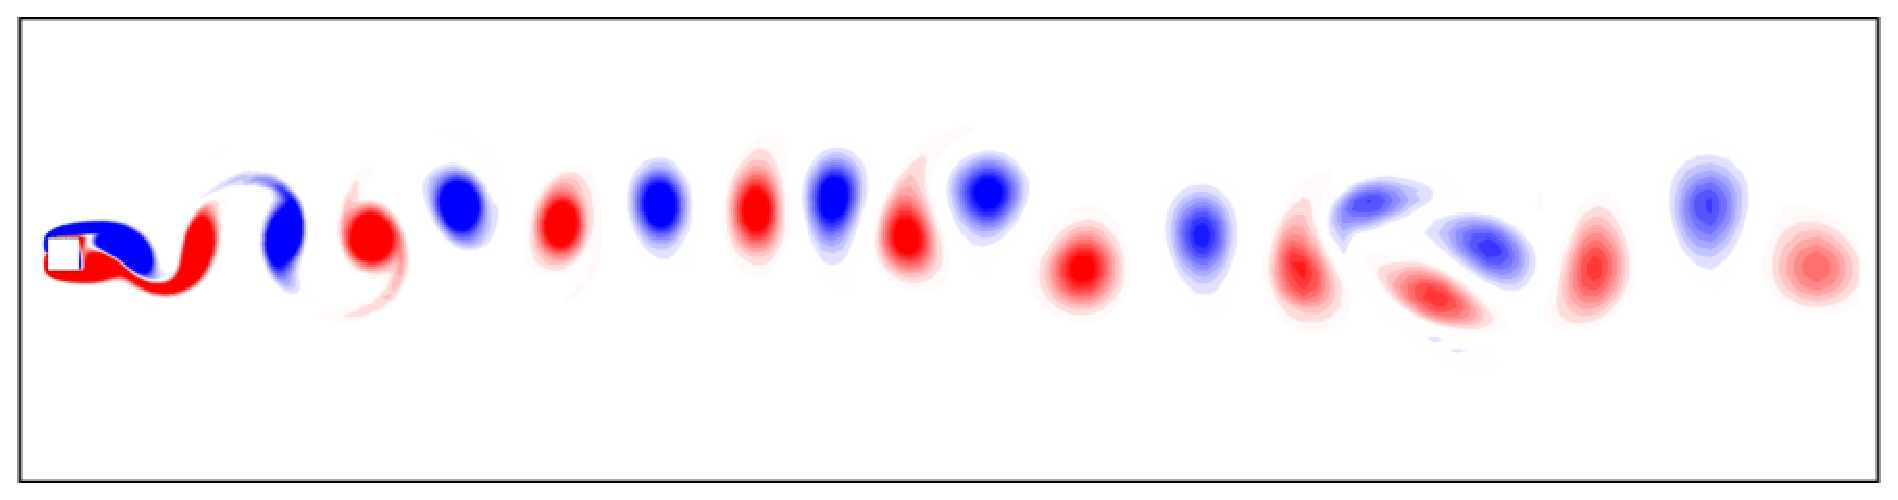
\includegraphics[width=1\unitlength]{../FnP/gnuplot/10.eps}}
    \put(0,1.22){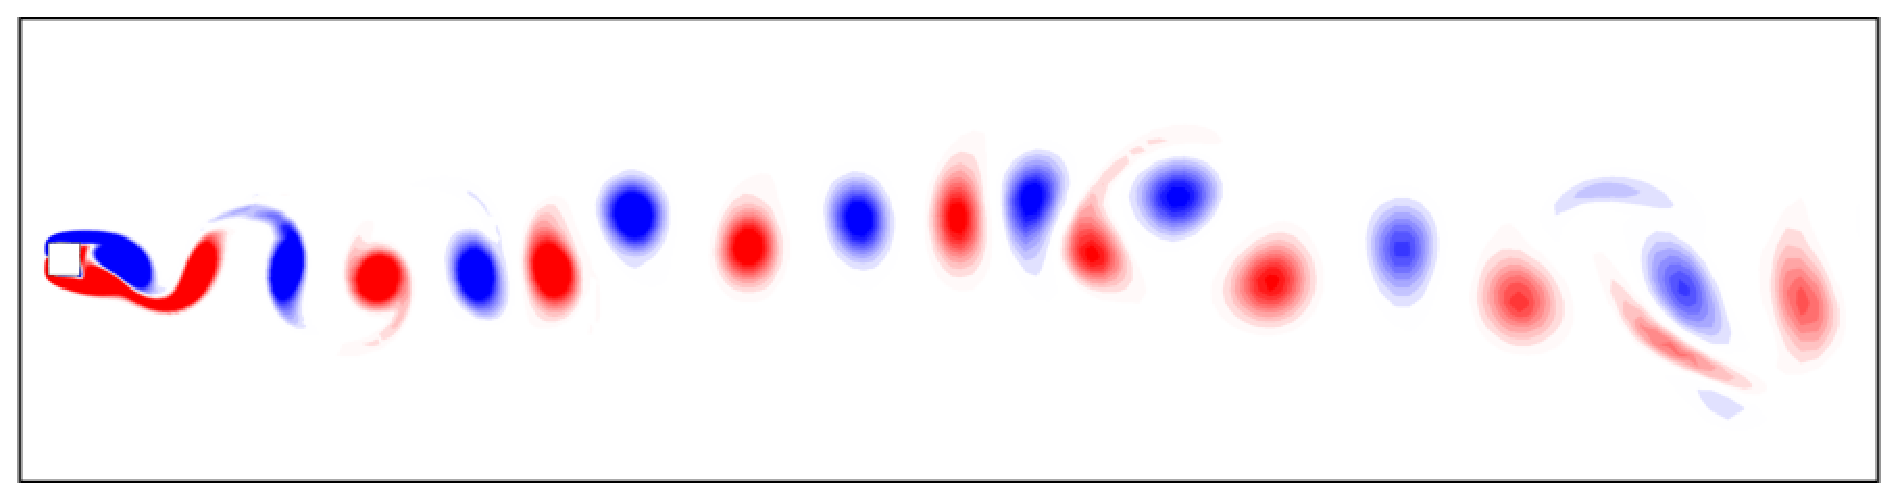
\includegraphics[width=1\unitlength]{../FnP/gnuplot/60.eps}}
    \put(0,0.94){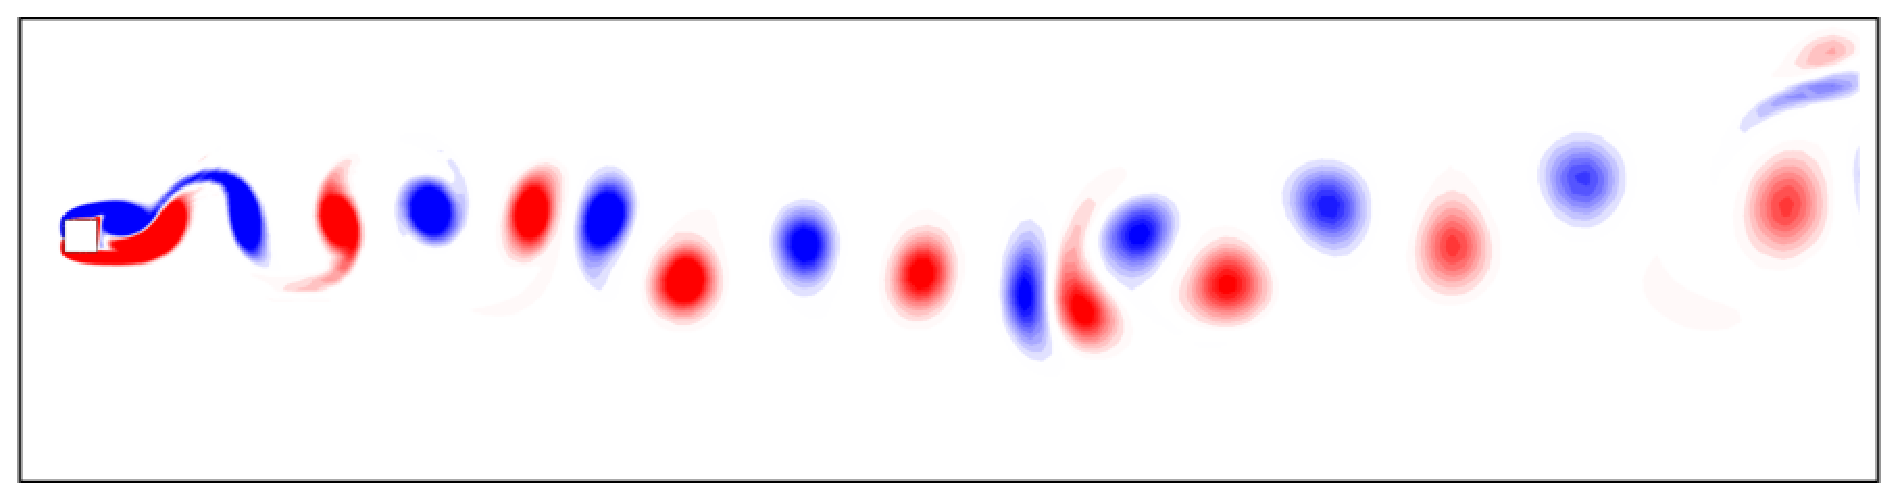
\includegraphics[width=1\unitlength]{../FnP/gnuplot/250.eps}}
    \put(0,0.66){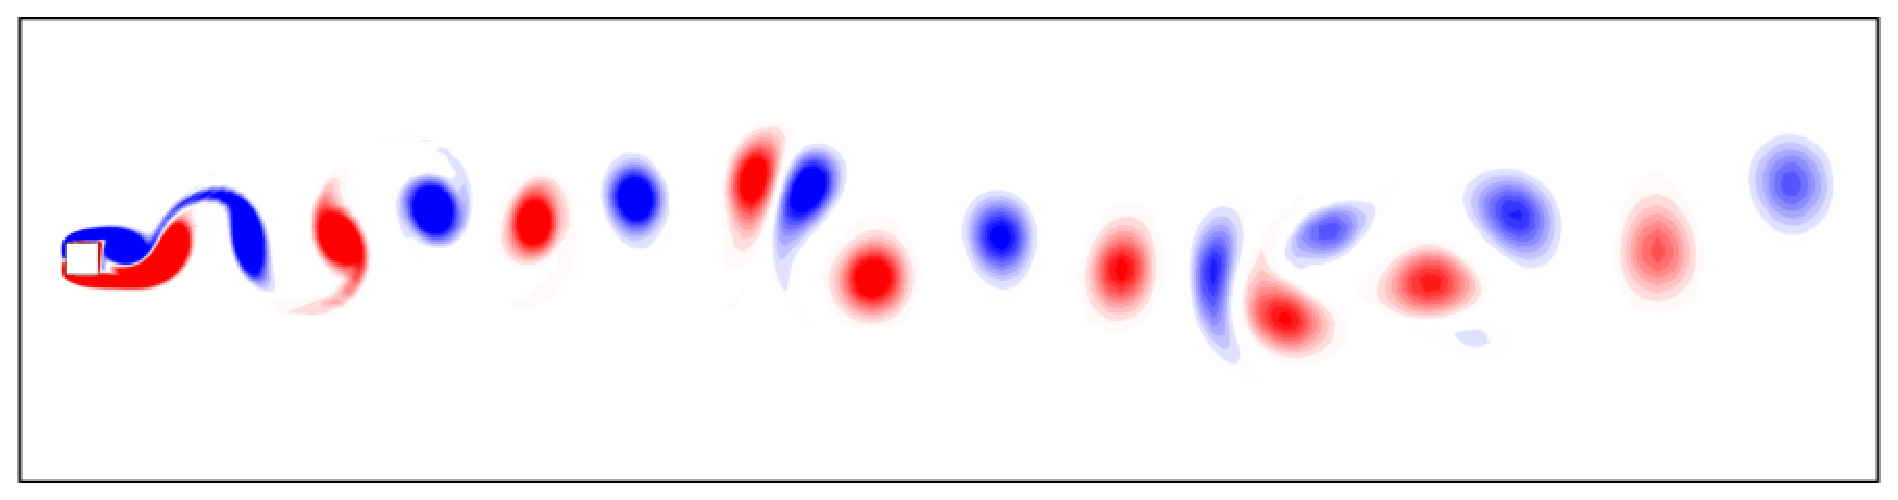
\includegraphics[width=1\unitlength]{../FnP/gnuplot/1000.eps}}

    \put(0.01,1.72){\small(a)}
    \put(0.01,1.44){\small(b)}
    \put(0.01,1.16){\small(c)}
    \put(0.01,0.88){\small(d)}
      
  \end{picture}

  \caption{Vorticity plots of the flow at arbitrary instants at
    $\massdamp=0.47$. (a) $\massstiff=10$, (b) $\massstiff=60$ (c)
    $\massstiff=250$ and (d) $\massstiff=1000$ at
    $\reynoldsnumber=200$. Contours show vorticity at levels between
    $\pm 1$.}
    \label{fig:flow_vis}
\end{figure}

 %vspace{10cm}




More information can be gained by analysing the flow field. Figure \ref{fig:flow_vis} shows the flow field data at arbitrary instances where the values of \massdamp\ are close to the point of the maximum power at different \massstiff\. A clear wavelength could be observed in this figure. Qualitatively, this can be interpreted as such that at high \massstiff, the vortex shedding is simply superimposed over the path of motion of the cylinder. A decrease in amplitude of this wave could be observed at low \massstiff\ which may be caused due to the higher levels of no-linear interactions between vortex shedding and galloping. Such an argument is conistant with the data of figure \ref{fig:spec_pow} that show the increasing significance of vortex shedding as \massstiff\ decreases. Bundled together, this also to a certain extent helps to explain the discrepancy between the mean extracted predicted by the QSS and DNS models at low \massstiff, highlighted in figure \ref{fig:error}.


\section{Summary of the governing parameters of  fluid-elastic galloping}
\label{sec:summary-pi_1-pi_2}

An analysis of the power transfer of a square body under fluid-elastic galloping is presented in this chapter. This analysis was carried out by solving the quasi-steady state oscillator model equation with the use of numerical integration. Dimensionless groups were formulated by through the relevant time scales by linearising the QSS equation. In comparison with classical VIV parameters i.e. $\zeta$ and \ustar a good collapse could be obtained with these newly formulated parameters. Having the collapsed data using the dimensionless groups further strengthens the argument that the velocity amplitude and the power transfer of the system does not depend on the natural frequency of the system over a large range of natural frequencies.


Although \mstar is shown to be an independent parameter in equation \ref{eqn:eom_nondim_regroup_pi_1_pi_2}, the results show that the system is only a function of \massstiff\ and \massdamp\ essentially. This could be explained by inspecting equation \ref{eqn:eom_nondim_regroup_pi_1_pi_2}, which shows that \mstar only has an impact on the forcing terms which are non-linear in relation to the velocity of the body. In order for these terms to be appreciable, the velocity of the body, and hence, the induced angle of attack need to be quite high, which e for the range of parameters tested here, appears not to be the case. 

Comparing with direct numerical simulation data, the quasi steady state model provide a good approximations of the power output when the \massstiff\ of the system is relatively large. But, at low values of \massstiff, the prediction has a large discrepancy, as the QSS model does not account for the impact of vortex shedding, where the influence increase as the \massstiff\ is decreased. That being said, the QSS model does provide quite a reasonable prediction of the value of \massstiff\ at the point where the maximum power is produced. Both the error in predicted maximum power between the QSS and the DNS models, and the relative power of the vortex shedding, have been quantified. It scale similarly to $1/\sqrt{\massstiff}$.

The presence of a clear wave length in the flow field at high \massstiff\ and the reduction of this wavelength as \massstiff\ decreases provides more evidence to the fact that vortex shedding has a complex influence on galloping systems.  





    


